% ============================================================================
% 附录 AE：动理学与回旋动理学：从弗拉索夫方程到回旋动理学（v1.26.9 新增）
%
% 数值唯一来源：tools/calc/appAE_calc.py → tools/calc/appAE_calc.txt（正文与门禁 P37 引用的
%   每一个数字都必须出现在该输出里；文献值只作定性对照，不参与数值断言）
% 单位写法：单位一律写进数学字体（\mathrm{...}），避免中文字符进数学模式
% 速度约定：v_the = sqrt(T_e/m_e)（与附录 AC 一致）、v_Ti = sqrt(2T_i/m_i)
%   （与附录 AD 的 rho_i 一致）、c_s = sqrt(T_e/m_i)（附录 AD 的离子声速）
% 版权口径：只借鉴结论、方程形式与题型；文字、数值、表格全部自拟，
%   由 tools/calc/appAE_calc.py 独立复算。离线环境无法核验 DOI，故只给书名/作者/年份/卷期页。
% 与其他附录的分工：附录 S 讲约束与输运（流体视角）、附录 AC 讲数值方法、
%   附录 W 讲快粒子与 alpha；本附录补「分布函数本身」这一层。
% ============================================================================

\section{分布函数：状态量为什么不能只是密度}
\label{sec:app-ae-distribution}

前面所有附录都默认一件事：等离子体可以用密度、温度、流速这几个数描述。
这在本附录要被打上一个条件——\textbf{只有碰撞足够频繁时，分布函数才会自己松弛到麦克斯韦分布}，
流体描述才是动理学方程的一个闭合近似。本附录先把「分布函数」这个状态量摆出来，
再一路走到回旋动理学：把最快的那个运动（回旋）平均掉，留下慢的漂移和湍流。

第一步是把速度空间的尺子摆好。三种速度刻度在本附录里反复出现，必须一开始就分清：

\begin{equation}
v_{the}=\sqrt{\frac{T_e}{m_e}}=4.02127\times10^{7}\ \mathrm{m\,s^{-1}}=0.134135c ,
\label{eq:app-ae-vthe}
\end{equation}

\begin{equation}
v_{Ti}=\sqrt{\frac{2T_i}{m_i}}=839.370\ \mathrm{km\,s^{-1}},\qquad
c_s=\sqrt{\frac{T_e}{m_i}}=593.524\ \mathrm{km\,s^{-1}} .
\label{eq:app-ae-vthe2}
\end{equation}

$v_{the}$ 取的是 $\sqrt{T_e/m_e}$ 口径（与附录 AC 的 $v_{the}$、$\Delta t$ 判据一致），
$v_{Ti}$ 取最概然速度口径（与附录 AD 的 $\rho_i$ 一致）；在 $T_i=T_e$ 时
$v_{Ti}=\sqrt{2}\,c_s$，两者不是同一个数。三种速度的用途也不同：
$v_{the}$ 管电子穿过网格与德拜球、$v_{Ti}$ 管离子轨道、$c_s$ 管离子声波与台基宽度。

\begin{table}[htbp]
\centering
\small
\begin{tabular}{p{3.0cm}p{3.4cm}p{3.2cm}p{4.4cm}}
\toprule
量 & 本工作点的值 & 表达式 & 它在哪件事里说话 \\
\midrule
电子热速度 & $4.02127\times10^{7}\ \mathrm{m\,s^{-1}}$ & $\sqrt{T_e/m_e}$ & 德拜判据、网格与时间步 \\
离子热速度 & $839.370\ \mathrm{km\,s^{-1}}$ & $\sqrt{2T_i/m_i}$ & 离子轨道、香蕉宽度 \\
离子声速 & $593.524\ \mathrm{km\,s^{-1}}$ & $\sqrt{T_e/m_i}$ & 离子声波、台基宽度 \\
德拜长度 & $71.2806\ \mathrm{\mu m}$ & $\sqrt{\epsilon_0T_e/(n_ee^2)}$ & 集体性判据、屏蔽 \\
德拜立方内粒子数 & $3.62171\times10^{7}$ & $n_e\lambda_{De}^3$ & 统计描述是否成立 \\
电子回旋半径 & $43.1386\ \mathrm{\mu m}$ & $v_{the}/\omega_{ce}$ & 电子尺度湍流 \\
离子回旋半径 & $4.13338\ \mathrm{mm}$ & $v_{Ti}/\omega_{ci}$ & 回旋动理学的展开参数 \\
\bottomrule
\end{tabular}
\caption{速度与长度刻度。$\rho_i/a=1/483.866$ 就是回旋动理学的展开参数：
它小，所以可以把回旋平均掉；它不为零，所以平均之后会留下有限拉莫尔半径效应。}
\label{tab:app-ae-scales}
\end{table}

德拜长度与德拜立方内粒子数决定了「能不能用统计量说话」：

\begin{equation}
\lambda_{De}=\sqrt{\frac{\epsilon_0T_e}{n_ee^2}}=71.2806\ \mathrm{\mu m},\qquad
n_e\lambda_{De}^3=3.62171\times10^{7} .
\label{eq:app-ae-debye}
\end{equation}

$3.62171\times10^{7}$ 这个数（与附录 AC 的 $N_D$ 同口径）说明两件事：
(1) 一个德拜球里粒子足够多，$f$ 的统计解释成立；
(2) 但它远小于宏观尺度，所以「多少算多」是尺度相对的——本工作点 $a/\lambda_{De}=2.80581\times10^{4}$。

两个回旋半径把电子和离子彻底分开：

\begin{equation}
\rho_e=\frac{v_{the}}{\omega_{ce}}=43.1386\ \mathrm{\mu m},\qquad
\rho_i=\frac{v_{Ti}}{\omega_{ci}}=4.13338\ \mathrm{mm},\qquad
\frac{\rho_i}{\rho_e}=95.8163 .
\label{eq:app-ae-rho}
\end{equation}

\begin{tip}{分布函数不是「更精确的密度」}{tip-app-ae-distribution}
$f(\mathbf{x},\mathbf{v},t)$ 不是把 $n(\mathbf{x},t)$ 加一个速度维度那么简单：它多出来的自由度
恰好承载了流体描述必须\textbf{假设}掉的东西——热流、黏性、各向异性、无碰撞阻尼。
所以凡是「平均自由程与梯度尺度可比」或「有粒子被俘获」的场合，流体方程不是近似得更差，
而是\textbf{结构性地缺项}。反过来，如果碰撞足够频繁，$f$ 自己会松弛到麦克斯韦分布，
流体方程不但够用，而且更省。判断用哪一套，靠的是本节的几个刻度，不是偏好。
\end{tip}

\textbf{出处：}动理学描述与德拜屏蔽的框架参照 Nicholson \emph{Introduction to Plasma Physics}
（1983，第 4--5 章）与 Chen \emph{Introduction to Plasma Physics and Controlled Fusion}
（第 2 版，1984，第 3 章）；速度分布的矩与闭合问题参照 Braginskii（1965，
\emph{Reviews of Plasma Physics} \textbf{1}, 205）与 Freidberg \emph{Ideal MHD}（2014，第 2 章）。

\section{无碰撞不等于无相互作用：弗拉索夫方程与闭合问题}
\label{sec:app-ae-vlasov}

无碰撞时 $f$ 满足弗拉索夫方程，它是「相空间里不可压缩」的另一种写法：

\begin{equation}
\frac{\partial f}{\partial t}+\mathbf{v}\cdot\nabla f+
\frac{q}{m}\left(\mathbf{E}+\mathbf{v}\times\mathbf{B}\right)\cdot\frac{\partial f}{\partial\mathbf{v}}=0 .
\label{eq:app-ae-vlasov}
\end{equation}

方程右端为零，不等于物理里没有相互作用：\textbf{平均场}已经被 $\mathbf{E}$、$\mathbf{B}$ 带进去了。
本工作点用三个乘积把这件事量化：

\begin{equation}
\omega_{pe}\tau_{ei}=5.03299\times10^{7},\qquad
\omega_{ce}\tau_{ei}=8.31634\times10^{7},\qquad
\omega_{ci}\tau_{ei}=18116.9 .
\label{eq:app-ae-collisionality}
\end{equation}

三个数都远大于 $1$：在一个回旋周期里，粒子几乎不可能被撞一次。等价的说法是平均自由程：

\begin{equation}
\lambda_{\mathrm{mfp}}=v_{the}\tau_{ei}=3.58755\ \mathrm{km},\qquad
\frac{\lambda_{\mathrm{mfp}}}{2\pi R}=92.0929 .
\label{eq:app-ae-mfp}
\end{equation}

一个热电子要沿着环绕 $92$ 圈才碰一次。用梯度尺度 $a$ 无量纲化，得到努森数

\begin{equation}
\mathrm{Kn}=\frac{\lambda_{\mathrm{mfp}}}{a}=1793.77,\qquad
\mathrm{Kn}_i=\frac{v_{Ti}\tau_{ii}}{a}=2536.78 ,
\label{eq:app-ae-kn}
\end{equation}

其中 $\tau_{ii}\simeq\tau_{ei}\sqrt{m_i/m_e}=6.04449\times10^{-3}\ \mathrm{s}$ 只作量级估计（声明值）。
$\mathrm{Kn}\gg1$ 意味着流体闭合在这里不是「精度差一点」，而是\textbf{必须显式引入}的东西。

\begin{table}[htbp]
\centering
\small
\begin{tabular}{p{3.6cm}p{3.0cm}p{3.4cm}p{4.0cm}}
\toprule
判据 & 本工作点 & 阈值 & 不成立时会发生什么 \\
\midrule
$\omega_{pe}\tau_{ei}$ & $5.03299\times10^{7}$ & $\gg1$ & 等离子体不屏蔽、像中性气体 \\
$\omega_{ce}\tau_{ei}$ & $8.31634\times10^{7}$ & $\gg1$ & 电子被磁化、回旋是快运动 \\
$\omega_{ci}\tau_{ei}$ & $18116.9$ & $\gg1$ & 离子未被电子碰撞钉住 \\
$\lambda_{\mathrm{mfp}}/(2\pi R)$ & $92.0929$ & $\gg1$ & 环向输运由轨道而非碰撞决定 \\
$\mathrm{Kn}=\lambda_{\mathrm{mfp}}/a$ & $1793.77$ & $\gg1$ & 流体闭合必须声明，不能默认 \\
\bottomrule
\end{tabular}
\caption{无碰撞判据。注意这些数不是「等离子体很稀」的同义词，而是「哪一个尺度上谁更快」的
比较：同一个工作点，在 $\rho_i$ 尺度上动理学效应很小，在 $\lambda_{\mathrm{mfp}}$ 尺度上却主导。}
\label{tab:app-ae-collisionless}
\end{table}

把 $f$ 的零阶、一阶、二阶矩取出来，就得到密度、流速与压强：

\begin{equation}
n=\int f\,d^3v,\qquad
\mathbf{u}=\frac{1}{n}\int\mathbf{v}f\,d^3v,\qquad
p=\frac{m}{3}\int(\mathbf{v}-\mathbf{u})^2f\,d^3v .
\label{eq:app-ae-moments}
\end{equation}

下一步的三阶矩就是热流，它出现在压强方程里，而压强方程又会牵出四阶矩——
这就是闭合问题。附录 S 用的都是已经闭合好的输运系数，本附录的价值在于说清
\textbf{那些系数是在什么假设下从 $f$ 里积出来的}。

\begin{tip}{无碰撞是个不等式，不是「没有相互作用」}{tip-app-ae-collisionless}
初学者常把「无碰撞」听成「粒子自由飞行、彼此无关」。但 $\omega_{ce}\tau_{ei}=8.31634\times10^{7}$
说的是「回旋比碰撞快八个量级」，而不是「没有碰撞」：碰撞仍然决定了长期的输运与弛豫，
只是它在短时间内可以忽略。真正被丢掉的是\textbf{短程二体碰撞}，保留下来的是平均场，
以及平均场与粒子之间的共振（下一节）。所以无碰撞等离子体里照样有耗散，
耗散机制从「碰撞」换成了「相混合」与「波粒共振」。
\end{tip}

\textbf{出处：}弗拉索夫方程与矩展开的写法参照 Nicholson \emph{Introduction to Plasma Physics}
（1983，第 6 章）与 Krall \& Trivelpiece \emph{Principles of Plasma Physics}（1973，第 3 章）；
闭合问题与 Braginskii 输运系数参照 Braginskii（1965，\emph{Reviews of Plasma Physics} \textbf{1}, 205）
与 Helander \& Sigmar \emph{Collisional Transport in Magnetized Plasmas}（2002，第 3--4 章）；
库仑对数与碰撞时间的量级参照 Wesson \emph{Tokamaks}（第 4 版，2011，第 14 章）。
本节凡标出数字的量都由 \texttt{tools/\allowbreak{}calc/\allowbreak{}appAE\_calc.py} 复算。
\section{波粒共振：Landau 阻尼为什么是「无碰撞」的}
\label{sec:app-ae-landau}

上一节的方程 (AE.5) 是可逆的：把时间倒过来，$f$ 会原路返回。可是等离子体里确实存在
\textbf{不可逆}的耗散——波会消失，而且没有一次碰撞。这件事的第一份定量答案是朗道给出的，
它的机制不是碰撞，而是\textbf{相混合}：不同速度的粒子以不同速率积累相位，
初始时相干的速度扰动被拉成越来越细的丝，任何有限分辨率的观测都再也看不到它。

能参与这件事的只有那些速度跟波的相速度同步的粒子，即 $v\approx v_{ph}=\omega/k$ 的共振粒子。
对麦克斯韦分布的朗缪尔波，无量纲阻尼率是

\begin{equation}
\frac{\gamma}{\omega}=-\sqrt{\frac{\pi}{8}}\,
\frac{1}{\left(k\lambda_{De}\right)^{3}}
\exp\!\left(-\frac{1}{2\left(k\lambda_{De}\right)^{2}}-\frac{3}{2}\right).
\label{eq:app-ae-landau}
\end{equation}

这个公式对 $k\lambda_{De}$ 极其敏感：

\begin{table}[htbp]
\centering
\small
\begin{tabular}{p{3.0cm}p{2.6cm}p{2.8cm}p{4.8cm}}
\toprule
模式 & $k\lambda_{De}$ & $\gamma/\omega$ & 读法 \\
\midrule
朗缪尔波 & $0.1$ & $-2.6969\times10^{-20}$ & 相速度远离尾部，几乎不衰减 \\
朗缪尔波 & $0.3$ & $-0.0200206$ & 已经能在一百个周期里看到衰减 \\
朗缪尔波 & $0.5$ & $-0.151387$ & 强阻尼，波只活几个周期 \\
朗缪尔波 & $1$ & $-0.0848088$ & 公式已越界（$\omega\simeq\omega_{pe}$ 不成立） \\
离子声波（$T_e/T_i=1$） & --- & $-0.094058$ & 离子声波靠电子与离子两头一起吃 \\
离子声波（$T_e/T_i=10$） & --- & $-0.00927902$ & 电子温度拉高，阻尼反而变弱 \\
\bottomrule
\end{tabular}
\caption{Landau 阻尼率。$10^{-20}$ 与 $10^{-1}$ 之间没有「差不多」：指数上的相速度
决定了一切。最后一行说明Landau 阻尼不是「温度越高越强」的单调故事。}
\label{tab:app-ae-landau}
\end{table}

取一个具体点：$k\lambda_{De}=0.3$ 时

\begin{equation}
\omega=\omega_{pe}\sqrt{1+3k^2\lambda_{De}^2}=6.3576\times10^{11}\ \mathrm{rad\,s^{-1}},\qquad
k=4208.72\ \mathrm{m^{-1}},\qquad
\lambda=1.4929\ \mathrm{mm},
\label{eq:app-ae-resonance}
\end{equation}

\begin{equation}
v_{ph}=\frac{\omega}{k}=1.51058\times10^{8}\ \mathrm{m\,s^{-1}}
=3.75648\,v_{the},\qquad
\exp\!\left(-\frac{v_{ph}^2}{2v_{the}^2}\right)=8.62603\times10^{-4} .
\label{eq:app-ae-resonance2}
\end{equation}

相速度落在热速度的 $3.76$ 倍处，处在麦克斯韦分布的尾巴上：速度超过 $v_{ph}$ 的电子只占
$2.75775\times10^{-3}$。Landau 阻尼吃掉的正是这一小撮——不是因为它多，而是因为它\textbf{不可替代}。

离子声波的情形多一层结构。它的相速度由 $c_s$ 决定，比离子热速度大、比电子热速度小，
于是电子和离子\textbf{同时}处在共振边缘：

\begin{equation}
T_e/T_i=1:\ \gamma/\omega=-0.094058;\qquad
T_e/T_i=10:\ \gamma/\omega=-0.00927902 .
\label{eq:app-ae-ionacoustic}
\end{equation}

在 $k\lambda_{De}=0.1$、$T_e/T_i=10$ 时，$k=1402.91\ \mathrm{m^{-1}}$、波长 $4.47869\ \mathrm{mm}$，
$\omega=kc_s=8.32659\times10^{8}\ \mathrm{rad\,s^{-1}}$，即 $f=132.522\ \mathrm{MHz}$。

\begin{tip}{Landau 阻尼不是「无碰撞的碰撞」}{tip-app-ae-landau}
把Landau 阻尼讲成「粒子像碰撞一样把波撞没了」会带来两个错误结论：
(1) 以为阻尼率随碰撞率增大而增大——恰恰相反，碰撞会把细丝抹平、\textbf{破坏}相混合；
(2) 以为它一定是耗散的——在非线性阶段，被困住的粒子可以把能量\textbf{还给}波，
这就是 BGK 模式与非线性朗道增长的来源。正确的图像是：
阻尼来自共振粒子的速度扩散（准线性理论），而能量的最终归宿是粒子还是波，
取决于分布函数的局部斜率——斜率反转时，阻尼就变成增长（不稳定性）。
\end{tip}

\textbf{出处：}Landau 阻尼的原始结果见 Landau（1946，\emph{Journal of Physics USSR}
\textbf{10}, 25）；「无碰撞阻尼」的物理解释与实验对照见 Jackson（1960，
\emph{Physics of Fluids} \textbf{3}, 786）与 Malmberg \& Wharton（1964，
\emph{Physical Review Letters} \textbf{13}, 184）；BGK 模式与非线性效应见 Bernstein,
Greene \& Kruskal（1957，\emph{Physical Review} \textbf{108}, 546）。
公式形式与量级参照 Nicholson \emph{Introduction to Plasma Physics}（1983，第 6--7 章）
与 Krall \& Trivelpiece \emph{Principles of Plasma Physics}（1973，第 8 章）。
本节凡标出数字的量都由 \texttt{tools/\allowbreak{}calc/\allowbreak{}appAE\_calc.py} 复算。

\section{捕获粒子、香蕉轨道与新经典输运}
\label{sec:app-ae-orbit}

把动理学放在托卡马克的几何里，第一个新东西是\textbf{磁镜}：环内侧磁场强、外侧弱，
于是速度方向与磁场夹角足够大的粒子会被反射，来回弹跳，无法绕环一整圈。
这些粒子叫捕获粒子，它们的轨道投影像香蕉。

先算三个几何刻度。反径比 $\epsilon=a/R=0.322581$、$\epsilon^{1.5}=0.183213$，
以及连接长度的一个尺度 $q_{95}R=21.7\ \mathrm{m}$。碰撞率与弹跳频率之比是判别输运区的关键：

\begin{equation}
\nu_*=\frac{\nu_{ei}\,qR}{\epsilon^{1.5}v_{the}}=0.0330145 .
\label{eq:app-ae-nustar}
\end{equation}

$\nu_*\ll1$ 就是\textbf{香蕉区}：粒子在被撞散之前，已经完成了许多次弹跳。
捕获比例由磁镜几何直接给出：

\begin{equation}
f_t=\sqrt{\frac{2\epsilon}{1+\epsilon}}=69.843\% .
\label{eq:app-ae-ftrap}
\end{equation}

接近七成的粒子是捕获粒子——这个数字常被低估，因为磁镜比的直觉容易让人以为
只有「贴着磁场大角度」的少数粒子会被抓。

\begin{equation}
\Delta_b=\frac{\rho_iq_{95}}{\sqrt{\epsilon}}=2.54715\ \mathrm{cm}
=6.16239\,\rho_i=1.27357\%\ \text{的 }a .
\label{eq:app-ae-banana}
\end{equation}

\begin{equation}
\omega_b=\frac{v_{Ti}\sqrt{\epsilon}}{q_{95}R}=21969.1\ \mathrm{s^{-1}},\qquad
f_b=3496.5\ \mathrm{Hz},\qquad
T_b=286.001\ \mathrm{\mu s} .
\label{eq:app-ae-bounce}
\end{equation}

香蕉宽度比回旋半径大 $6$ 倍——这不是小修正，而是\textbf{新经典输运的几何来源}：
粒子在一个弹跳周期内横向走出 $2.5\ \mathrm{cm}$，它的漂移不再被回旋运动平均掉。
同理，捕获粒子与通行粒子之间的摩擦会产生自举电流（附录 S 里的那部分）。

\begin{table}[htbp]
\centering
\small
\begin{tabular}{p{3.2cm}p{3.0cm}p{3.4cm}p{4.2cm}}
\toprule
量 & 本工作点 & 表达式 & 它在哪件事里说话 \\
\midrule
反径比 $\epsilon$ & $0.322581$ & $a/R$ & 磁镜深度 \\
碰撞率 $\nu_*$ & $0.0330145$ & $\nu_{ei}qR/(\epsilon^{1.5}v_{the})$ & 输运区判别（$<1$ 香蕉区） \\
捕获比例 $f_t$ & $69.843\%$ & $\sqrt{2\epsilon/(1+\epsilon)}$ & 有多少粒子在弹跳 \\
香蕉宽度 $\Delta_b$ & $2.54715\ \mathrm{cm}$ & $\rho_iq_{95}/\sqrt{\epsilon}$ & 新经典输运的步长 \\
弹跳频率 $f_b$ & $3496.5\ \mathrm{Hz}$ & $v_{Ti}\sqrt{\epsilon}/(2\pi q_{95}R)$ & 弹跳周期 $286\ \mathrm{\mu s}$ \\
\bottomrule
\end{tabular}
\caption{轨道刻度。三个数必须一起看：$\nu_*$ 决定「是不是香蕉区」，
$f_t$ 决定「有多少粒子在弹跳」，$\Delta_b$ 决定「跳一步有多宽」。}
\label{tab:app-ae-orbit}
\end{table}

\begin{tip}{香蕉轨道不是「轨道」，是漂移的平均失败}{tip-app-ae-orbit}
单粒子轨道图上看，香蕉轨道是一条闭合的「香蕉」。但它在输运里的作用不是「多了一条轨道」，
而是「原本应该被回旋平均掉的垂直漂移，现在平均不掉了」：
通行粒子上行与下行各走半圈，漂移方向相反、相互抵消；
捕获粒子的上下两段是同一个方向，抵消失败。所以新经典输运把经典值抬高了
$\sim1/\sqrt{\epsilon}$ 倍，而这个因子在本工作点是 $1.76068$。
\end{tip}

\textbf{出处：}香蕉轨道与新经典输运的框架见 Galeev \& Sagdeev（1968，
\emph{Reviews of Plasma Physics} \textbf{7}, 257）；系统的综述见 Hinton \& Hazeltine
（1976，\emph{Reviews of Modern Physics} \textbf{48}, 239）与 Helander \& Sigmar
\emph{Collisional Transport in Magnetized Plasmas}（2002，第 6--8 章）；
自举电流与捕获粒子的关系参照 Wesson \emph{Tokamaks}（第 4 版，2011，第 4 章）。
本节凡标出数字的量都由 \texttt{tools/\allowbreak{}calc/\allowbreak{}appAE\_calc.py} 复算。
\begin{figure}[htbp]
\centering
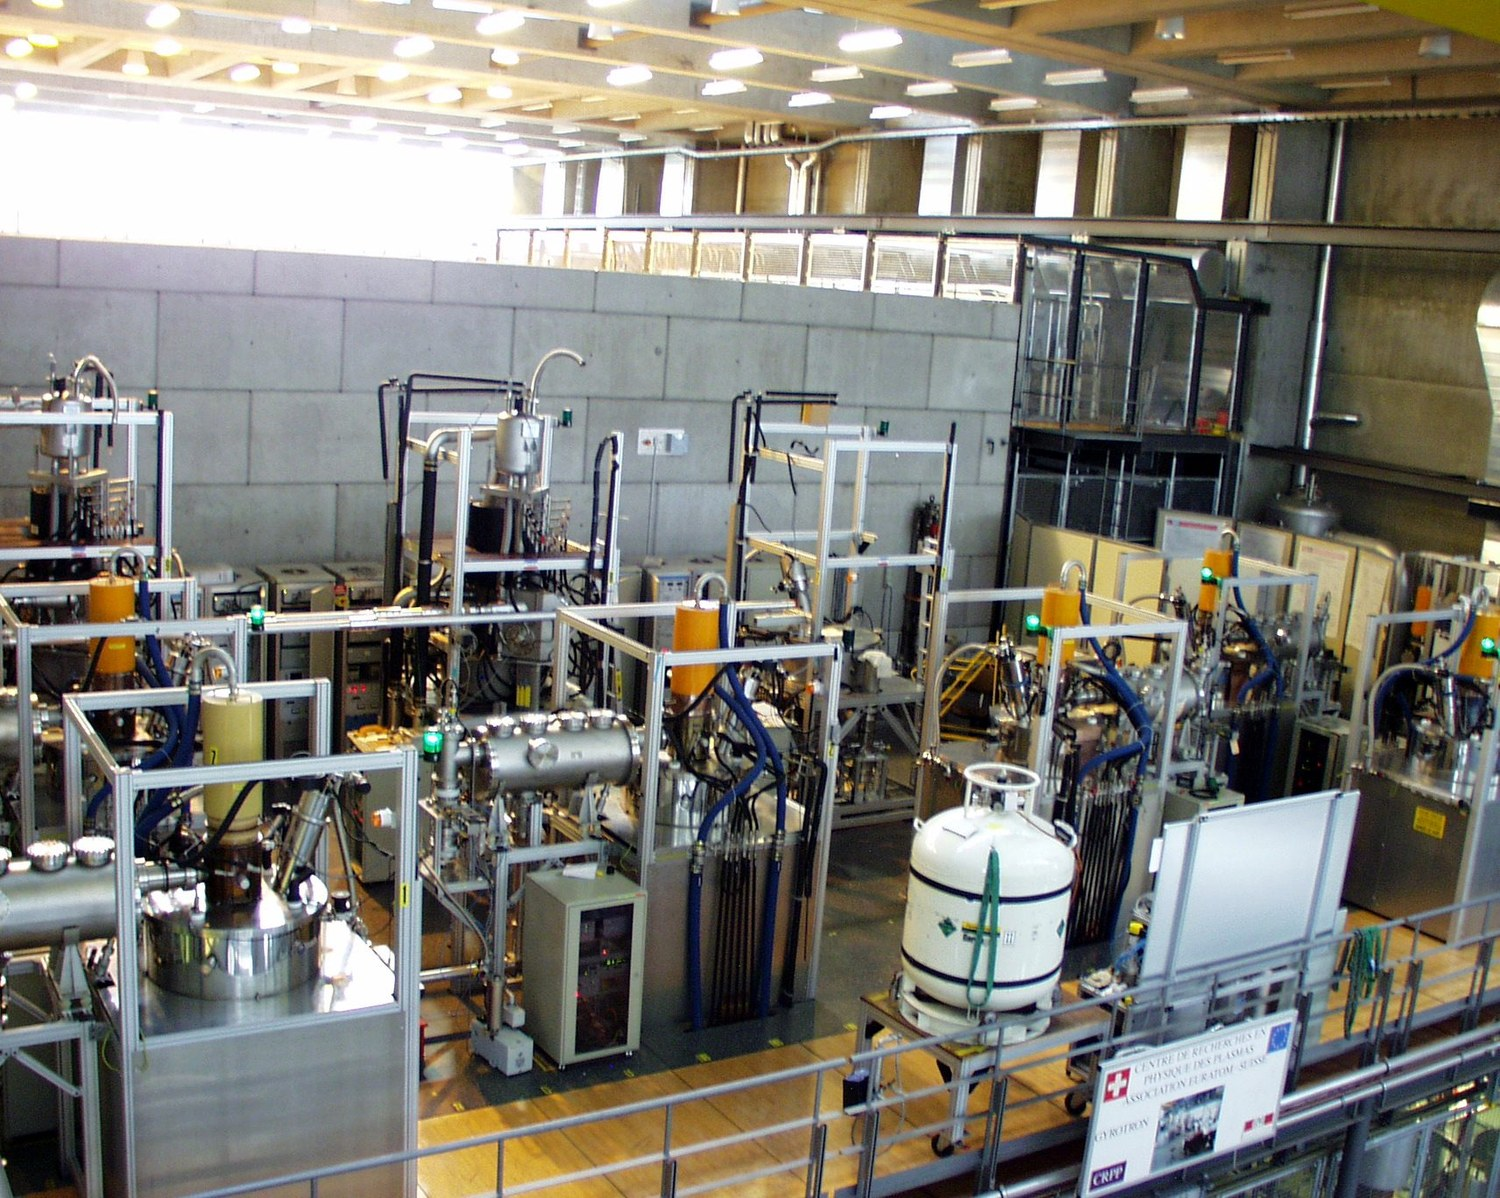
\includegraphics[width=0.78\textwidth]{../figures/ae_gyrotron.jpg}
\caption{把电子回旋运动当快变量平均掉，才有回旋动理学；回旋管则反过来利用这段运动做毫米波源。本节出现的回旋频率与回旋半径，正是这台器件的工作参数。}
\label{fig:photo-appae2}
\figsource{Rama，CC BY-SA 2.5（Wikimedia Commons）}
\end{figure}

\section{回旋动理学：把最快的那个运动平均掉}
\label{sec:app-ae-gyro}

带电粒子在磁场里最快的运动是回旋。本工作点

\begin{equation}
\frac{\rho_i}{a}=\frac{1}{483.866}=2.0668\times10^{-3},\qquad
\left(\frac{\rho_i}{a}\right)^{2}=4.2712\times10^{-6},
\label{eq:app-ae-gyro}
\end{equation}

也就是说，离子回旋半径比装置小两个多量级。这就是回旋动理学的\textbf{展开参数}：
既然回旋又快又小，就把回旋相位当成一个可以平均掉的「内部变量」，
只留下回旋中心（导心）的运动。平均不是免费的，代价是分布函数降维之后
出现的有限拉莫尔半径（FLR）效应：

\begin{equation}
\Gamma_0(b)=I_0(b)e^{-b},\qquad b=k_\perp^2\rho_i^2 .
\label{eq:app-ae-gamma0}
\end{equation}

取 $k_\perp\rho_i=0.3$（本工作点最典型的湍流尺度）：

\begin{equation}
k_\perp=72.5799\ \mathrm{m^{-1}},\qquad
\lambda_\perp=8.65693\ \mathrm{cm},\qquad
k_\perp\rho_e=0.00313099 .
\label{eq:app-ae-gyro2}
\end{equation}

同一个波长下，电子几乎感觉不到这个尺度（$k_\perp\rho_e\approx0.003$），
所以「离子尺度湍流」这个说法是有依据的：它选择性地作用在离子通道上。

\begin{table}[htbp]
\centering
\small
\begin{tabular}{p{2.4cm}p{2.6cm}p{3.0cm}p{5.2cm}}
\toprule
$k_\perp\rho_i$ & $b$ & $\Gamma_0(b)$ & 抑制掉的比例 $1-\Gamma_0$ \\
\midrule
$0.3$ & $0.09$ & $0.915783$ & $8.42172\%$（长波，FLR 只是修正） \\
$1$ & $1$ & $0.46576$ & $53.424\%$（一半以上的响应被抹平） \\
$2$ & $4$ & $0.207002$ & $79.2998\%$（短波，几乎完全被平均掉） \\
\bottomrule
\end{tabular}
\caption{有限拉莫尔半径因子。$\Gamma_0$ 随 $b$ 单调下降：$k_\perp\rho_i$ 越大，
回旋平均抹掉的东西越多。这就是回旋动理学与漂移波理论之间的连接点。}
\label{tab:app-ae-gyro}
\end{table}

把 $\rho_i$、$c_s$、$a$ 组合起来，就得到回旋玻姆扩散系数，它是本附录里
「湍流输运」的标尺：

\begin{equation}
\chi_{gB}=\frac{\rho_i^2c_s}{a}=5.07013\ \mathrm{m^2\,s^{-1}},\qquad
\chi_{B}=\frac{T_e}{16eB}=108.42\ \mathrm{m^2\,s^{-1}},\qquad
\frac{\chi_B}{\chi_{gB}}=21.384 .
\label{eq:app-ae-chigb}
\end{equation}

玻姆扩散比回旋玻姆大 $21$ 倍，这是「最坏情况」的粗略估计。
反过来，用能量约束时间反推的有效扩散系数

\begin{equation}
\chi_{\mathrm{eff}}=\frac{a^2}{2\tau_E}=0.540541\ \mathrm{m^2\,s^{-1}},\qquad
\frac{\chi_{\mathrm{eff}}}{\chi_{gB}}=0.106613,\qquad
\frac{\chi_B}{\chi_{\mathrm{eff}}}=200.577
\label{eq:app-ae-chieff}
\end{equation}

（$\tau_E=3.7\ \mathrm{s}$ 是声明值，与附录 AD 的同一工作点一致）说明：
这个工作点的输运比回旋玻姆\textbf{好} $9.37973$ 倍，比玻姆好 $200$ 倍。
「等离子体为什么比玻姆扩散好」是约束物理的核心问题之一，回旋动理学是回答它的工具。

\begin{tip}{回旋动理学不是「把回旋平均掉就完事」}{tip-app-ae-gyro}
如果回旋真的可以被完全平均掉，等离子体就退化成一组沿磁场滑动的导心，
回旋半径会从方程里彻底消失——那也就没有 FLR 效应、没有回旋阻尼、
没有耗散性的潜在机制。回旋动理学\textbf{保留}回旋半径的一阶效应
（$k_\perp\rho_i$ 的有限值、$\Gamma_0$、回旋黏性），只丢掉回旋相位的快变部分。
所以它不是一个「近似更差的 Vlasov」，而是一个\textbf{被系统降维、同时保留关键物理}的模型：
计算量从六维相空间降到五维，代价是必须正确处理 $\Gamma_0$ 这类平均后的算符。
\end{tip}

\textbf{出处：}回旋动理学的系统推导见 Frieman \& Chen（1982，\emph{Physics of Fluids}
\textbf{25}, 502）与 Antonsen \& Lane（1980，\emph{Physics of Fluids} \textbf{23}, 1205）；
现代综述见 Brizard \& Hahm（2007，\emph{Reviews of Modern Physics} \textbf{79}, 421）；
回旋玻姆与玻姆标度的对照、以及离子尺度湍流的输运定标参照 Hahm \& Burrell
（1995，\emph{Physics of Plasmas} \textbf{2}, 1648）；$\Gamma_0$ 因子的写法与
回旋黏性参照 Helander \& Sigmar \emph{Collisional Transport in Magnetized Plasmas}
（2002，第 6 章）。本节凡标出数字的量都由 \texttt{tools/\allowbreak{}calc/\allowbreak{}appAE\_calc.py} 复算。

\section{速度分布的形状：尾部、损失锥与从动理学到流体}
\label{sec:app-ae-tail}

动理学的全部信息都在 $f$ 的形状里。本节用三个问题把形状量化：
尾巴有多厚、损失锥吃掉多少、以及什么时候可以丢掉 $f$ 只用流体量。

麦克斯韦分布的尾部按 $\exp(-u^2)$ 衰减，$u=v/v_{the}$：

\begin{equation}
u>1:\ 57.2407\%,\qquad
u>2:\ 4.60117\%,\qquad
u>3:\ 0.043985\%,\qquad
u>4:\ 5.23347\times10^{-5}\% .
\label{eq:app-ae-tail}
\end{equation}

换成能量口径（$T_e=9.194\ \mathrm{keV}$）：

\begin{equation}
E>10\ \mathrm{keV}:\ 53.6824\%,\qquad
E>64\ \mathrm{keV}:\ 0.30131\%,\qquad
E>100\ \mathrm{keV}:\ 7.34126\times10^{-5}\% .
\label{eq:app-ae-energytail}
\end{equation}

$57\%$ 的电子跑得比「热速度」快——因为热速度是分布的宽度而不是上限；
但真正决定核反应率的是 $10$ 倍热速度以上的部分。
$3.5\ \mathrm{MeV}$ 的 alpha 粒子（$v=1.29472\times10^{7}\ \mathrm{m\,s^{-1}}
=15.4249\,v_{Ti}$）如果硬要当作热尾，它的权重是 $\exp(-u^2)=4.67\times10^{-104}$：
一个在任何计算机里都等于零的数。\textbf{所以聚变产物必须单独当成一个分量处理}——
这正是附录 W 要做的事。

损失锥是形状问题的另一个侧面。磁镜比 $R_m$ 决定锥角 $\theta_c=\arcsin(R_m^{-1/2})$：

\begin{equation}
R_m=2:\ \theta_c=45^\circ,\ 29.2893\%;\qquad
R_m=5:\ \theta_c=63.4349^\circ,\ 10.5573\% .
\label{eq:app-ae-losscone}
\end{equation}

括号里的百分数是各向同性分布中落入损失锥的比例
（$1-\sqrt{1-1/R_m}$）：磁镜比越大，被反射的越多、漏出去的越少。
$3.5\ \mathrm{MeV}$ alpha 的回旋半径是 $5.10055\ \mathrm{cm}=12.3399\,\rho_i$——
比热离子的轨道大一个量级，所以快粒子不能被当作「更热的背景」。

\begin{table}[htbp]
\centering
\small
\begin{tabular}{p{3.4cm}p{3.2cm}p{3.0cm}p{4.2cm}}
\toprule
分布特征 & 本工作点 & 表达式 & 后果 \\
\midrule
$v>v_{the}$ & $57.2407\%$ & 高斯尾 & 一半以上粒子「比热速度快」 \\
$v>3v_{the}$ & $0.043985\%$ & 高斯尾 & 电流、射频共振的作用区间 \\
$E>64\ \mathrm{keV}$ & $0.30131\%$ & 能量尾 & 与 $T_e$ 的比决定反应率 \\
alpha 等效 $u$ & $15.4249$（$v_{Ti}$） & $v_\alpha/v_{Ti}$ & 热尾权重 $4.67\times10^{-104}$ \\
损失锥（$R_m=2$） & $29.2893\%$ & $1-\sqrt{1-1/R_m}$ & 磁镜泄漏份额 \\
\bottomrule
\end{tabular}
\caption{分布函数的形状。前四行说明「尾部决定反应率」，最后一行说明
「几何决定泄漏」。两者都不能用平均值代替。}
\label{tab:app-ae-velocity}
\end{table}

最后一个问题是：什么时候可以扔掉 $f$，只用流体量？判据是努森数与碰撞率：

\begin{equation}
\mathrm{Kn}=1793.77,\qquad
\lambda_{\mathrm{mfp},i}=5.07356\ \mathrm{km},\qquad
\mathrm{Kn}_i=2536.78 ,
\label{eq:app-ae-closure}
\end{equation}

\begin{equation}
\frac{\kappa_\perp}{\kappa_\parallel}\sim\frac{1}{\left(\omega_{ce}\tau_{ei}\right)^{2}}
=1.44589\times10^{-16}\quad\text{(电子)},\qquad
\frac{1}{\left(\omega_{ci}\tau_{ii}\right)^{2}}=6.63719\times10^{-13}\quad\text{(离子)} .
\label{eq:app-ae-anisotropy}
\end{equation}

前一组说明「必须用动理学」；后一组说明「平行与垂直方向差十几个数量级，
所以流体闭合必须写成张量，不能写成标量」。附录 S 用的各向异性输运系数，
就是在这个夹缝里被构造出来的。

\begin{tip}{聚变靠的是尾部，不是平均能量}{tip-app-ae-tail}
每次听到「等离子体温度是一亿度」，都值得换算一下尾部：$9.194\ \mathrm{keV}$ 的
平均能量对应的 D-T 反应率，靠的是 $E>64\ \mathrm{keV}$ 的那 $0.3\%$；
如果分布只是「平均值对」，形状错了，反应率可以差一个量级。
反过来，诊断量（中子率、聚变功率）是尾部加权量，而压强、储能是矩加权量——
两者对 $f$ 的敏感程度完全不同。这就是为什么动理学诊断（中子谱、charge exchange）
与流体诊断必须一起看。
\end{tip}

\textbf{出处：}麦克斯韦分布尾部与矩的关系见 Nicholson \emph{Introduction to Plasma Physics}
（1983，第 4 章）；D-T 反应率对温度的依赖参照 Bosch \& Hale（1992，
\emph{Nuclear Fusion} \textbf{32}, 611）；alpha 粒子慢化与快粒子分量参照
Wesson \emph{Tokamaks}（第 4 版，2011，第 1、14 章）；损失锥与磁镜的经典处理
见 Krall \& Trivelpiece \emph{Principles of Plasma Physics}（1973，第 1 章）；
各向异性输运与张量闭合参照 Braginskii（1965，\emph{Reviews of Plasma Physics} \textbf{1}, 205）。
本节凡标出数字的量都由 \texttt{tools/\allowbreak{}calc/\allowbreak{}appAE\_calc.py} 复算。
\section{估算练习}
\label{sec:app-ae-problems}

以下六题都可以只用本附录的公式与本工作点参数手算。答案保留四到六位有效数字，
每一步都能用 \texttt{tools/\allowbreak{}calc/\allowbreak{}appAE\_calc.py} 复算。

\textbf{练习 1}（尺度换算）把工作点换成 $n_e=1\times10^{19}\ \mathrm{m^{-3}}$、
$T_e=T_i=1\ \mathrm{keV}$、$B=5.3\ \mathrm{T}$：求德拜长度、德拜立方内粒子数、
离子热速度与离子回旋半径，并说明 $a/\rho_i$ 变成多少。

\textbf{练习 2}（FLR 因子）取 $k_\perp\rho_i=1$：求 $k_\perp$、垂直波长、
$\Gamma_0(1)$ 以及被抑制掉的比例。再回答：为什么电子对同一波长的响应几乎不受影响？

\textbf{练习 3}（尾部）本工作点 $T_e=9.194\ \mathrm{keV}$，求 $v>3v_{the}$ 的电子比例，
以及 $1\ \mathrm{m^3}$ 里有多少个这样的电子。

\textbf{练习 4}（无碰撞判据）把密度降到 $n_e=1\times10^{19}\ \mathrm{m^{-3}}$
（$\tau_{ei}\propto1/n_e$）：求碰撞时间、平均自由程，以及 $\lambda_{\mathrm{mfp}}/(2\pi R)$。

\textbf{练习 5}（香蕉宽度）安全因子从 $q_{95}=3.5$ 换成 $q=1.7$：香蕉宽度变成多少？
与原来相差几倍？

\textbf{练习 6}（快粒子）$3.5\ \mathrm{MeV}$ 的 alpha 粒子：速度是 $v_{Ti}$ 的几倍？
如果把它塞进麦克斯韦分布，热尾权重 $\exp(-u^2)$ 是多少？回旋半径是 $\rho_i$ 的几倍？

\textbf{解答 1} 德拜长度 $\lambda_{De}=7.43394\times10^{-5}\ \mathrm{m}=74.3394\ \mathrm{\mu m}$
（比工作点略长，因为 $T_e$ 低了近一个量级、$n_e$ 低了一个量级）；
德拜立方内粒子数 $n_e\lambda_{De}^3=4.10826\times10^{6}$（仍远大于 $1$）；
离子热速度 $v_{Ti}=276822\ \mathrm{m\,s^{-1}}$、$\rho_i=1.36318\ \mathrm{mm}$，
于是 $a/\rho_i=1467.16$——比工作点小了三倍，回旋动理学的展开仍然很好用。

\textbf{解答 2} $k_\perp=1/\rho_i=241.933\ \mathrm{m^{-1}}$，
$\lambda_\perp=2\pi/k_\perp=0.0259708\ \mathrm{m}=2.59708\ \mathrm{cm}$，
$\Gamma_0(1)=0.46576$，抑制掉 $53.424\%$。电子几乎不受影响是因为
$k_\perp\rho_e=k_\perp\rho_i\cdot(\rho_e/\rho_i)=1/95.8163=0.0104366$，
$\Gamma_0$ 在这个小量下接近 $1$。

\textbf{解答 3} $v>3v_{the}$ 的比例是 $0.043985\%$，即
$n_e\times4.3985\times10^{-4}=4.3985\times10^{16}\ \mathrm{m^{-3}}$。
尾部只有万分之四，但它决定了束-等离子体不稳定性与射频共振的位置。

\textbf{解答 4} $\tau_{ei}=8.92144\times10^{-4}\ \mathrm{s}$（密度降十倍，碰撞时间涨十倍），
$\lambda_{\mathrm{mfp}}=v_{the}\tau_{ei}=35875.5\ \mathrm{m}=35.8755\ \mathrm{km}$，
$\lambda_{\mathrm{mfp}}/(2\pi R)=920.929$——比工作点的 $92$ 倍又稀了十倍。

\textbf{解答 5} $\Delta_b=\rho_iq/\sqrt{\epsilon}=0.0123719\ \mathrm{m}=1.23719\ \mathrm{cm}$，
是 $q_{95}=3.5$ 时 $2.54715\ \mathrm{cm}$ 的 $1/2.05882$。
安全因子越低，香蕉轨道越窄，新经典输运的步长越小——但 $q$ 也影响稳定性，
所以「把 $q$ 压到最低」并不是免费的。

\textbf{解答 6} $v_\alpha=1.29472\times10^{7}\ \mathrm{m\,s^{-1}}=15.4249\,v_{Ti}$，
热尾权重 $\exp(-u^2)=4.67\times10^{-104}$（在任何浮点格式里都是零），
回旋半径 $\rho_\alpha=5.10055\ \mathrm{cm}=12.3399\,\rho_i$。
结论：alpha 粒子必须作为一个独立分量求解，不能用背景分布的尾部代替。

\section{来源、分级与版权说明}
\label{sec:app-ae-source}

本附录的数值分三级，读者可以据此判断每个数有多「硬」：

(1) \textbf{现算级}：由 \texttt{tools/\allowbreak{}calc/\allowbreak{}appAE\_calc.py} 从工作点参数直接算出，
包括所有速度、长度、频率、比例与本节的练习解答。这一级的每一个数字都可在脚本里复现。

(2) \textbf{声明级}：脚本顶部的输入与约定，包括 $\tau_E=3.7\ \mathrm{s}$、
$\ln\Lambda=17$、$\tau_{ii}=\tau_{ei}\sqrt{m_i/m_e}$、$T_e=T_i$、
捕获粒子公式的几何假设、损失锥比例用的各向同性分布假设。
它们不是从第一性原理算出来的，而是本附录明确选择的口径。

(3) \textbf{文献级}：只作定性对照、不参与任何数值断言，例如Landau 阻尼的原始文献、
回旋动理学的推导文献、D-T 反应率的拟合文献。离线环境无法核验 DOI，
所以只给作者、书名或刊名、年份与卷期页。

\begin{table}[htbp]
\centering
\small
\begin{tabular}{p{4.0cm}p{4.4cm}p{5.0cm}}
\toprule
来源 & 借鉴了什么 & 不借用什么 \\
\midrule
Nicholson (1983)；Chen (1984) & 动理学框架、德拜屏蔽、矩与闭合的讲法 & 原书文字、编号、插图、习题 \\
Krall \& Trivelpiece (1973) & 弗拉索夫方程、Landau 阻尼、磁镜的处理 & 原书推导步骤与符号体系 \\
Landau (1946)；Jackson (1960) & Landau 阻尼的结论与物理图像 & 原文推导与实验数据点 \\
Malmberg \& Wharton (1964) & 「无碰撞阻尼可观测」这一事实 & 实验曲线与数值 \\
Bernstein, Greene \& Kruskal (1957) & 非线性（BGK）图像 & 原文构造细节 \\
Brizard \& Hahm (2007) & 回旋动理学的现代综述框架 & 综述的章节结构与公式编号 \\
Hahm \& Burrell (1995) & 回旋玻姆与玻姆标度的对照 & 定标拟合系数 \\
Galeev \& Sagdeev (1968)；Hinton \& Hazeltine (1976) & 香蕉轨道与新经典输运的结论 & 原综述的推导与图表 \\
Helander \& Sigmar (2002) & 输运系数与张量闭合的口径 & 原书公式编号与数据 \\
Wesson (2011) & 工作点参数、快粒子与 alpha 的地位 & 原书表格与数值 \\
Bosch \& Hale (1992) & D-T 反应率对温度的依赖 & 拟合公式与系数 \\
\bottomrule
\end{tabular}
\caption{本附录的文献来源与借用边界。本附录的文字、数值、表格与练习全部自拟，
由 \texttt{tools/\allowbreak{}calc/\allowbreak{}appAE\_calc.py} 独立复算；文献只提供结论与图像。}
\label{tab:app-ae-source}
\end{table}

本附录明确声明四条\textbf{不复制}：

(1) 不复制任何教材或综述的文字、编号、插图与数据表；

(2) 不复制经典文献里的推导细节，只采用已被广泛引用的结论与量级；

(3) 不引用任何实验数据点、拟合曲线或软件输出作为本附录的数值来源——
所有数字都能在 \texttt{tools/\allowbreak{}calc/\allowbreak{}appAE\_calc.py} 里找到对应的一行；

(4) 不复制任何软件的文档或教程；工具层面的入门由附录 G 承担，本附录只讲方法。

\begin{tip}{诚实地说清「本附录不给什么」}{tip-app-ae-honest}
本附录给的是\textbf{标度、判据与量级}，不是回旋动理学方程的数值解，
也不是湍流谱或输运系数的第一性原理预测。具体地说：
(1) 不给 $\chi_{\mathrm{eff}}$ 的从微波到湍流的推导，只给它与回旋玻姆的比值；
(2) 不给非线性Landau 阻尼的饱和谱；(3) 不给损失锥不稳定性的增长率。
这些都需要真正的回旋动理学代码，属于附录 AC 讲的方法范畴。
把边界写清楚，比让读者以为「公式一贴就能预测约束时间」要诚实得多。
\end{tip}

\textbf{出处：}本节的文献清单与版权口径参照本教材其他附录的惯例
（见附录 X、附录 AB 的来源节）；工作点参数与附录 AC、附录 AD、附录 S 保持一致，
以便跨附录对照。本节不含任何由脚本复算的数字。
